\chapter{Metodi}

\subsection{BLAST}
Poređenje dve sekvence može se raditi na nivou nukleotida ili na nivou proteina. Poređenje na nivou proteina može pomoći u otkrivanju važnih bioloških informacija. Takođe, mnoge mutacije u DNK se ne odražavaju na nivou proteina i ne dovode do bilo kakve promene u odgovarajućoj amino kiselini. Shodno tome, za daleke odnose između organizama sa malom identičnošću sekvence na nivou DNK, poređenje proteina je bolje.


\subsection{Objašnjenje}
BLAST je skraćenica od Basic Local Alignment Search Tool koji su dizajnirali Eugene Myers, Stephen Altschul, Warren Gish, David J. Lipman i Webb Miler. Kao što samo ime kaže zasniva se na lokalnom poravnanju niski proteina ili amino kiselina. BLAST je značajno brži od običnog Smith-Waterman algoritma i od FASTA metoda (kasnije naveden). Heurističkim algoritmima upoređuje datu nisku sa bazama. Ne ocenjuje poklapanje i neslaganje univerzalno, nego po nekim statistikama izračuna značajnost konkretnih slaganja/neslaganja i pomoću njih izračunava ukupnu ocenu. Na osnovu toga kako su zadati ulazni podaci i kakvu bazu potražujemo, BLAST metode možemo da kategorišemo u pet potkategorija:
\begin{enumerate}
\item Nukleotid BLAST: DNK nisku uporedi sa DNK bazom podataka
\item Protein BLAST: nisku proteina uporedi sa proteinskom bazom podataka
\item Blastx: datu DNK sekvencu prevodi na šest mogućih načina u nisku proteina i to uporedi sa proteinskom bazom podataka
\item Tblastn: datu sekvencu proteina uporedi sa DNK bazom podataka, tako da DNK niske iz baze prevede u nisku  proteina
\item Tblastx: i zadatu DNK nisku i DNK niske prevede prvo u niske proteina pa posle ih upoređuje
\end{enumerate} \vspace{5mm}

Prilikom korišćenja algoritma koristimo neke bitne parametre:

\begin{enumerate}
\item Očekivan prag: (E-value odn. E-vrednost) predstavlja očekivan broj slučajnih pogodaka kod traženja u bazi. Za BLAST je E-vrednost obično 10.
\item Veličina reči: (k) algoritam je osnovan na k-merima. Obično  se kod proteina koriste 3-meri (kod manjih peptida nekad 2-meri) a kod aminokiselina 11-meri (vrednost može da varira između 7 i 15). Što kraće k-mere koristimo to precizniji rezultat dobijemo ali gubimo na vremenu potrebnom za pretragu baze podataka.
\item Matrica skora: Kada su niske aminokiselina u pitanju, izborom nekog od pre opisanih matrica PAM ili BLOSUM (u zavisnosti od prirode problema) ocenjujemo pogodke, pomašaje i praznine. Kod niske nukleotida obično pogodak (match) se boduje sa "+1", promašaj (mismatch) "-2" a praznine linearno, bez kažnjavanja ulazka u prazninu.
\item Prag T: prag se odnosi na skor kod traženja poravnanja prvog k-mera. Što veći T to precizniji rezultat, ali može da previdi neke moguće k-mere.
\end{enumerate} \vspace{5mm}

BLAST algoritam prvo podeli niske na k-mere, pa prilikom traženja nađe ne samo one niske koje se preklapaju slovo po slovo, nego i one koje sadrže neki promašaj slova. 
U sledećem primeru VLD poravnamo sa VLE. Pogledamo sve 3-mere od kojih najveći skor ima KYN sa KYN. Proširimo poravnanje levo i desno.

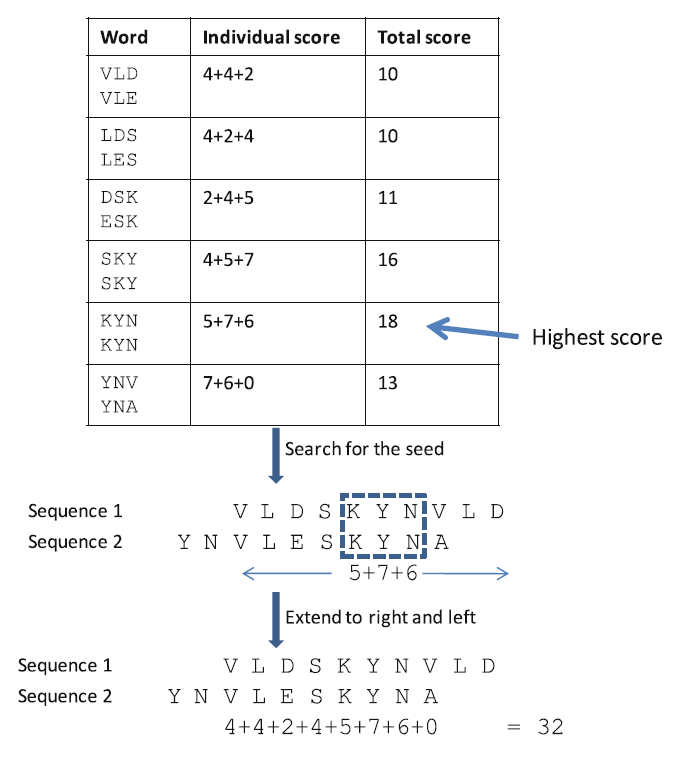
\includegraphics{blast}

\subsection{PSI-BLAST}
Vrsta BLAST metode za traženje proteina koji su slični ali u manjoj meri. Specifičnost ove varijante metoda je da matrica skora zavisi od pozicije u niski.

\subsection{PHI-BLAST}
Specializovan BLAST koji omogućava traženje šeme u bazi podataka. Na primer jedno parče aminokiseline koje je korisno kod identifikacije proteinske porodice.

\section{FASTA}
Slično kao BLAST, radi sa k-merima (obično 1-2 kod proteina i 4-6 kod nukleotida) i traži pogodke koji su blizu, povezuje ih ali bez uvođenja praznina, i na osnovu povezanih regija izračuna neku inicijalnu ocenu. U sledećem koraku program izabere 10 najboljih regija i sa običnim Smith-Waterman algoritmom traži poravnanje u parovima.

\subsection{Metode i alate}

\subsection{MegaBLAST}
Program kod NCBI koji je prilagođen traženju jako sličnih DNK seknvence. Brži je od običnog BLAST-a zato što veličina reči kod uparivanja je visoka, obično 28 a u nekim slučajevima je čak 64 karaktera. Druga specifičnost koji utiče na brzinu je da praznine kažnjava na uniformalan način. (nema razlike kod otvaranja praznine)

\subsection{BLAT}
Program je napravljen za poravnanje dugačkih DNK niski sa minimum 95% poklapanjem za vrlo brzo vreme.

\subsection{BLATZ}
Program traži ponovjene regije u prvom genomu, koje su prisutne i u dugom genomu. Briše ove regije. Posle traži niske od 19 nukleotida od kojih je minimum 12 pogodaka u poravnanju. Ove niske nastavi da proširi bez praznine dok ocena poravnanja ne preskoči neki definisan prag.

\subsection{LAGAN}
Veoma efikasan alat za poravnanje dve niske. Prvo potraži jedno optimalno lokalno poravnanje, koji služi kao temelj daljeg algoritma CHAOS. CHAOS traži kratke niske koje se ne moraju slovo po slovo preklapati. Na osnovu prethodnih generiše jednu grubu globalnu mapu, pa na kraju finalno poravnanje.

\subsection{MUMMER}
Alat koji radi lokalno poravnanje pomoću sufiksnih stabala. Poznat je po tome da nalazi sve posebne podniske sa velikom efikasnošću i među njima izabere maksimalne jedinstvene takozvane MUM-ove (Maximal Unique Match). U sledećem koraku izdvoji najduže koji pripadaju u oba genoma a regije među njima poravna Smith-Waterman algoritmom.

\subsection{Mugsy}
Jedan od alata koji poravna više genoma u isto vreme. Koristi se za traženje duplikacija ili delova gde se desilo premeštanje u genomu.

\subsection{WABA}
Program se koristi kad je u pitanju poravnanje dugačkih niski. Traži niske od 6 karaktera, na osnovu šeme 11011011 nađe inicijalne pogotke, gde 1 mora da bude pogodak(match). Ovako efikasno radi sa indelima. (insertion i deletion)
